Consider the following class diagram candidates:

\figureSeriesHere{}{\figureSeriesRow{\figureSeriesElement{1}{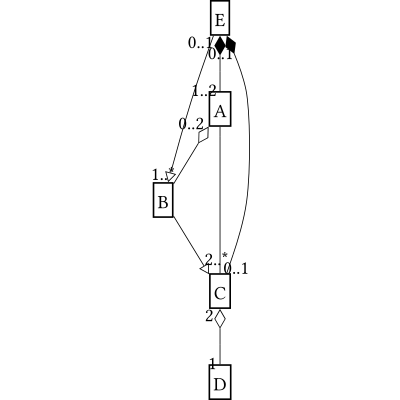
\includegraphics[min width=0.5\textwidth,min height=0.4\textwidth,max width=\textwidth,max height=\textwidth]{51/cdd1c5ae472de9a69c41400d40945817ce0c09750e9729e833d60a4440b740670400af83b04c596701db35357ce8aed00a3a92e08161.pdf}}}\figureSeriesRow{\figureSeriesElement{2}{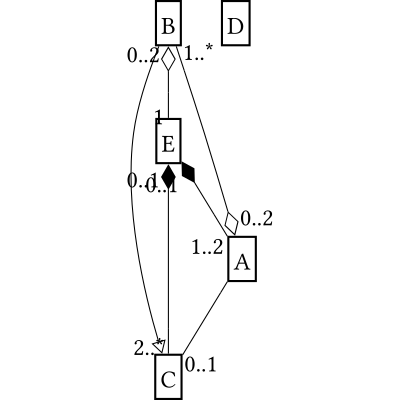
\includegraphics[min width=0.5\textwidth,min height=0.4\textwidth,max width=\textwidth,max height=\textwidth]{51/cd32786ed7955f75f2e4050d7464df637cf40075b2d129bb678089584e2eed975200af83b04c596701db35357ce8aed00a3a92e08161.pdf}}}\figureSeriesRow{\figureSeriesElement{3}{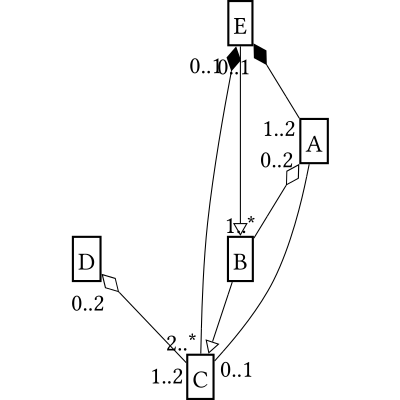
\includegraphics[min width=0.5\textwidth,min height=0.4\textwidth,max width=\textwidth,max height=\textwidth]{51/cdc2b5c869c289558f837f2bfe49d32b0e3b89293a325e08146a4a4c80b59e35fe00af83b04c596701db35357ce8aed00a3a92e08161.pdf}}}\figureSeriesRow{\figureSeriesElement{4}{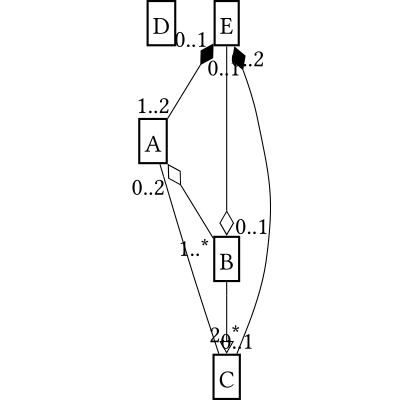
\includegraphics[min width=0.5\textwidth,min height=0.4\textwidth,max width=\textwidth,max height=\textwidth]{51/cd3faf14323c0cc9a0be4d24da2f2bee302bf2951cb8edca73b19f0e1599317b0300af83b04c596701db35357ce8aed00a3a92e08161.pdf}}}}Which of these class diagram candidates are valid class diagrams?
Please state your answer by giving a list of numbers, indicating all valid class diagrams.

For example,
\begin{minted}{text}
[1, 2]
\end{minted}
would indicate that only class diagram candidates 1 and 2 of the given ones are valid class diagrams.

Please note: Classes are represented simplified here. 
 That means they consist of a single box containing only the class name but no sections for attributes or methods. 
 Nevertheless you should treat these simplified class representations as valid classes.

Please note: When hovering over or clicking on edges / nodes or their labels, the respective components that belong together are highlighted.

